\documentclass[12pt,a4paper,titlepage]{scrreprt}
\usepackage[utf8]{inputenc}
\usepackage[english]{babel}

\usepackage[natbib=true,style=authoryear-ibid]{biblatex}
\usepackage{url}
\usepackage{hyperref}
\usepackage{fancyvrb}
\usepackage{csquotes}
\usepackage{upquote}

\usepackage{amsmath}
\usepackage{amssymb}

\newcommand{\catC}{\mathbb{C}}
\newcommand{\opcat}[1]{{#1}^{\text{op}}}
\newcommand{\Sets}{\mathbf{Sets}}

\DefineVerbatimEnvironment{code}{Verbatim}{fontsize=\small}

\hypersetup{
    colorlinks,
    linkcolor=black,
    citecolor=black,
    filecolor=black,
    urlcolor=black
}

\bibliography{literature}

\title{Cat-arrows}
\author{%
    Johannes Emerich
        (\href{mailto:Johannes@emerich.de}{johannes@emerich.de})\\
    Ignas Vyšniauskas
        (\href{mailto:i.vysniauskas@gmail.com}{i.vysniauskas@gmail.com})
}
\date{}

\begin{document}


\maketitle

\begin{abstract}
    This is a report on Arrows.
\end{abstract}

\section{Context}
\begin{frame}
\frametitle{Liberating Programming from the ``von Neumann'' style}

\begin{itemize}
    \item John Backus' call for new language paradigm (1978)
    \begin{itemize}
        \item \emph{Functional} programming (``FP'') as combinatorial
              approach to program construction
        \item Construct programs in an algebra of programs
        \item Variables range over \emph{programs}, operations are \emph{on}
              programs (\emph{pointfree} style)
        \item Functional style: only one state transition per operation
    \end{itemize}
    \item Haskell as most popular language true to Backus' ideas
\end{itemize}
\end{frame}

\begin{frame}
\frametitle{Haskell is non-strict}

\begin{columns}[c]
    \begin{column}{.6\textwidth}
        \begin{itemize}
            \item Problem of functions in computing: non-termination
            \item \emph{Lift} all types by adding an \texttt{undefined} ($\bot$) bottom
                  element, lowest in information order
            \item Set $B = \{\textrm{True}, \textrm{False}\}$ lifted to $B_\bot
                  = B \cup \{\bot\}$
            \item Functions are $B_\bot \to B_\bot$
        \end{itemize}
    \end{column}
    \begin{column}{.4\textwidth}
        \begin{center}
        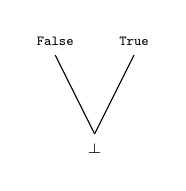
\begin{tikzpicture}
            \draw[font=\tiny] (0,0) node[below] {$\bot$} -- (0.5,1) node[above] {\texttt{True}};
            \draw[font=\tiny] (0,0) -- (-0.5,1) node[above] {\texttt{False}};
        \end{tikzpicture}
        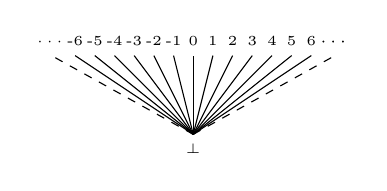
\begin{tikzpicture}
            \draw[dashed, font=\tiny] (0,0) -- (1.8,1) node[above] {$\cdots$};
            \draw[font=\tiny] (1.8,1) node[above] {$\cdots$};
            \draw[font=\tiny] (0,0) -- (1.5,1) node[above] {6};
            \draw[font=\tiny] (0,0) -- (1.25,1) node[above] {5};
            \draw[font=\tiny] (0,0) -- (1.0,1) node[above] {4};
            \draw[font=\tiny] (0,0) -- (0.75,1) node[above] {3};
            \draw[font=\tiny] (0,0) -- (0.5,1) node[above] {2};
            \draw[font=\tiny] (0,0) -- (0.25,1) node[above] {1};
            \draw[font=\tiny] (0,0) node[below] {$\bot$} -- (0,1) node[above] {0};
            \draw[font=\tiny] (0,0) -- (-0.25,1) node[above] {-1};
            \draw[font=\tiny] (0,0) -- (-0.5,1) node[above] {-2};
            \draw[font=\tiny] (0,0) -- (-0.75,1) node[above] {-3};
            \draw[font=\tiny] (0,0) -- (-1,1) node[above] {-4};
            \draw[font=\tiny] (0,0) -- (-1.25,1) node[above] {-5};
            \draw[font=\tiny] (0,0) -- (-1.5,1) node[above] {-6};
            \draw[dashed, font=\tiny] (0,0) -- (-1.8,1) node[above] {$\cdots$};
        \end{tikzpicture}
        \end{center}
    \end{column}
\end{columns}
\end{frame}

\begin{frame}[fragile]
\frametitle{Haskell is non-strict}
\begin{itemize}
    \item \emph{Strict} semantics
          \[
            \forall f: A_\bot \to B_\bot, f(\bot) = \bot
          \]
    \item Non-strict semantics allow operating on (potentially) infinite data
          structures:
          \begin{center}\verb|or ([True] ++ repeat False) == True|\end{center}
    \item Expressions only partially evaluated (\emph{thunks}) until value needed
    \item Problem for effectful computations whose result is never
          needed, e.g.
          \begin{center}\verb|print "Hello, Dave!"|\end{center}
\end{itemize}
\end{frame}

\begin{frame}[fragile]
\frametitle{Haskell is pure}
\begin{itemize}
    \item Functions are mappings from domain to codomain
    \item Haskell functions are \emph{pure}, they are \emph{only} mappings
    \item No side-effects (input/output, changes to global state)
    \item Beneficial for achieving Backus' desiderata
    \item But side-effects are desirable feature of programs
    \item How to bring them back in?
\end{itemize}
\end{frame}

\begin{frame}[fragile]
\frametitle{Computational lambda-calculus and monads}
\begin{itemize}
    \item Eugenio Moggi ('89): program equivalence in $\lambda$-calculus
    \item Semantics for \emph{general} notion of computation
          \begin{itemize}
              \item Side-effects, non-determinism, non-termination
          \end{itemize}
    \item Categorical language semantics with types as objects
          \begin{itemize}
              \item Distinguish type $B$ from corresponding \emph{computations} $TB$
              \item Model each notion of computation as a monad
          \end{itemize}
    \item Adopted into Haskell as general interface to computation
          \begin{itemize}
              \item Functions have to be pure, computations don't
          \end{itemize}
\end{itemize}
\end{frame}


\printbibliography

\end{document}
